\documentclass[12pt]{article}
\usepackage{amsmath}
\usepackage{amssymb}
\usepackage{float,graphicx}
\usepackage{hyperref}
\usepackage[latin1]{inputenc}
\usepackage{enumitem}
\usepackage{amsthm}
\usepackage{fancyvrb}
\usepackage[euler]{textgreek}

\hypersetup{
    colorlinks=true,
    linkcolor=blue,
    filecolor=magenta,      
    urlcolor=cyan,
}


\title{CSE 138 Lab 4}
\author{
  Matan Broner\\
  \and
  Krshant Chettiar\\
  \and 
  Kenneth Tang
}
\date{12/11/2020}

\begin{document}
\maketitle

\section{Objective}
Design and implement a key-value store that is partition-tolerant, available, and causally consistent. The key-value store is expected to be available even during a partition and must specifically provide causal consistency. Keys are partitioned into shards to achieve scalability and each shard must be replicated to ensure that the KVS is fault tolerant.
\newline
To achieve these objectives, the following mechanisms are required:
\begin{enumerate}
	\item A mechanism to ensure causal consistency even during partitions
	\item A mechanism to ensure eventual consistency even during partitions

\end{enumerate}

\section{Technologies Used}
\begin{enumerate}
	\item Docker
	\item Python 3.8, Flask
\end{enumerate}

\section{Workflow}
Clients are able to communicate with the key-value store through a dedicated API. The API is able to accept requests through the following routes:
\begin{enumerate}
	\item Key manipulation:
	\begin{verbatim}
		/kvs/keys/<key>
	\end{verbatim}
	This route allows for GET, PUT, and DELETE requests, allowing users to read, manipulate, and remove key value pairs from the store.
	\item Key count:
	\begin{verbatim}
		/kvs/key-count
	\end{verbatim}
	Allows a client to query the number of key-value pairs stored at a given node in the network.
	\item View change:
	\item \begin{verbatim}
		/kvs/view-change
	\end{verbatim}
	Allows a client to inform the network of a change in "view", meaning that the current set of active nodes in the network has been changed.
	\item \begin{verbatim}
		/kvs/shards
	\end{verbatim}
	Retrieves information for all shards in the KVS. Response contains the id of all shards.
	\item \begin{verbatim}
		/kvs/shards/<id>
	\end{verbatim}
	Retrieves information for a specific shard. Returns the number of keys and which replica it is stored on.
\end{enumerate}
\section{Causal Consistency}
Causal consistency states that all causally related operations should be read in the same order across a system. The following are guaranteed by causal consistency:
\begin{enumerate}
	\item Events that manipulate data and are causally related must be seen by all nodes in the same order
	\item Concurrent events that modify data may be seen in a different order
	\item Nodes should respond to reads only if client has knowledge of earlier events

\end{enumerate}
\textbf{Data Structure}
\newline
To implement causal consistency in a KVS, causal context is required. Causal-context represents the history of the data operations, which means the client has already witnessed all the events carried by causal-context. The following data structure is carried in the causal-context and is used to maintain causal consistency across the key-value store: 
\begin{verbatim}
[
    ["a", {
    "cause": [["b", 1594370977.537462]],
    "deleted": false,
    "last-write": 1607370977.5734642
    }]
]
\end{verbatim}

In the above case, key a is caused by the write of b in the given timestamp. Note that a being dependent on b indicates that b was either written before writing a, read before writing a, or deleted before writing a. The KVS's mechanism will verify that during the reading of a key, each causal write in each item in the given causal context is available in the given replica. If the key in question does not belong to the shard in which that replica is placed, the replica will query the correct shard to which that key is hashed and will verify that a timestamp for the last write of that key is later or equal. In short, if b belongs to the replica receiving the request, the replica will verify that it has seen an equal to or later write to b, and if not, the replica will ask b's corresponding shard if it can provide an equal to or later write for b. Failing to fulfil the correct case will result in a 400 being returned to the client, indicating a causal consistency error.

Every event that modifies data will return a causal context with the above data structure. The cause field keeps track of all events that are causally related to a given event. The last-write is used to keep track of the last-write for the key-value that the client has witnessed. The last-write field is used for breaking ties when there are concurrent requests. The deleted field is used to track whether a key has been deleted or not.
\newline
\newline
\textbf{Requests}
\newline
A brief description of requests that affect causality in the KVS.
\begin{enumerate}
\item{PUT and DELETE Requests}
\newline
Any client regardless of its causal context can make a successful PUT or DELETE request as all requests that modify data are made later than any that node has witnessed.  For DELETE requests to work successfully, a field in the causal-context data structure. The “deleted” field as implied by its name, keeps track of whether a value has been deleted or not. This field is required even events that have been deleted still may be relevant when relating events causally. 

\item{GET Request}
\newline
For a GET request to be successful, it either needs to have no causal-context (not witnessed any events) or it needs to have causal-context that is later than that of the key-value it is trying to read. If a client has causal-context that has knowledge of all earlier events, it is successfully able to read. If it does not have knowledge of earlier events, the node responds with “Unable to satisfy request”. If a client has the proper causal-context required to read a value and if a node must act as a proxy, it will always get back the latest value for a given key even if gossiping has not yet occurred.
\end{enumerate}
\makebox[\linewidth]{
  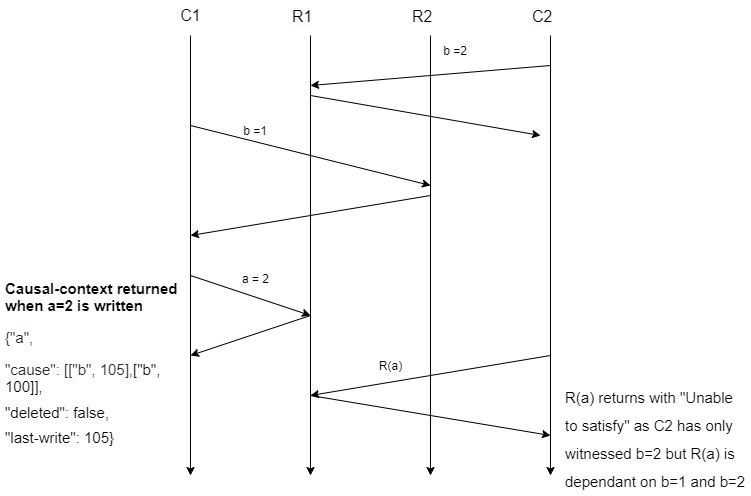
\includegraphics[keepaspectratio=true,scale=0.5]{assets/causal.jpeg}}
\section{Eventual Consistency}
When there are no network partitions, all replicas should converge to newest, correct state. To do this, a gossip protocol must be implemented for replicas to exchange state. A scheduler is used to ensure gossiping between nodes and replicas occur every 5 seconds. If a node and its corresponding replica have different states for the same key, both will have to agree and end up with the same final state. To do this, the state with the latest causal context is used or in the case of concurrent events, the key with the latest last write is chosen.
\makebox[\linewidth]{
  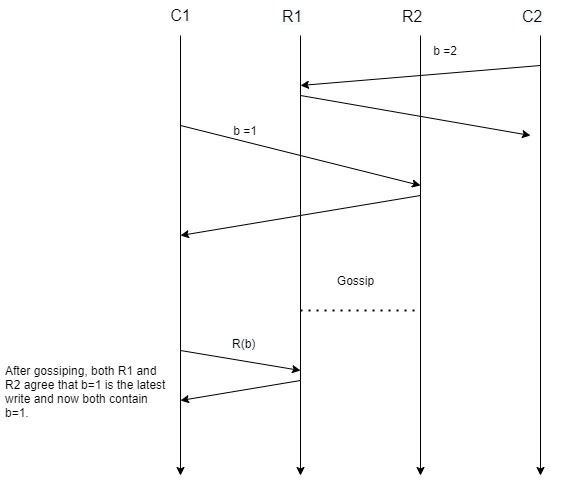
\includegraphics[keepaspectratio=true,scale=0.5]{assets/gossip.jpeg}}
\section{Unit Testing}
Aside from using the provided test scripts from the course TA, our group created  python scripts to test causality and gossiping with various node and replication factor configurations. 


\end{document}
